\chapter{図表の配置}
\label{ch:figure_table}



\section{図の配置}
\label{sec:figure}


\subsection{図を一枚だけ配置する方法}
\label{ssec:figure_sigle}

\begin{figure}
    \centering
    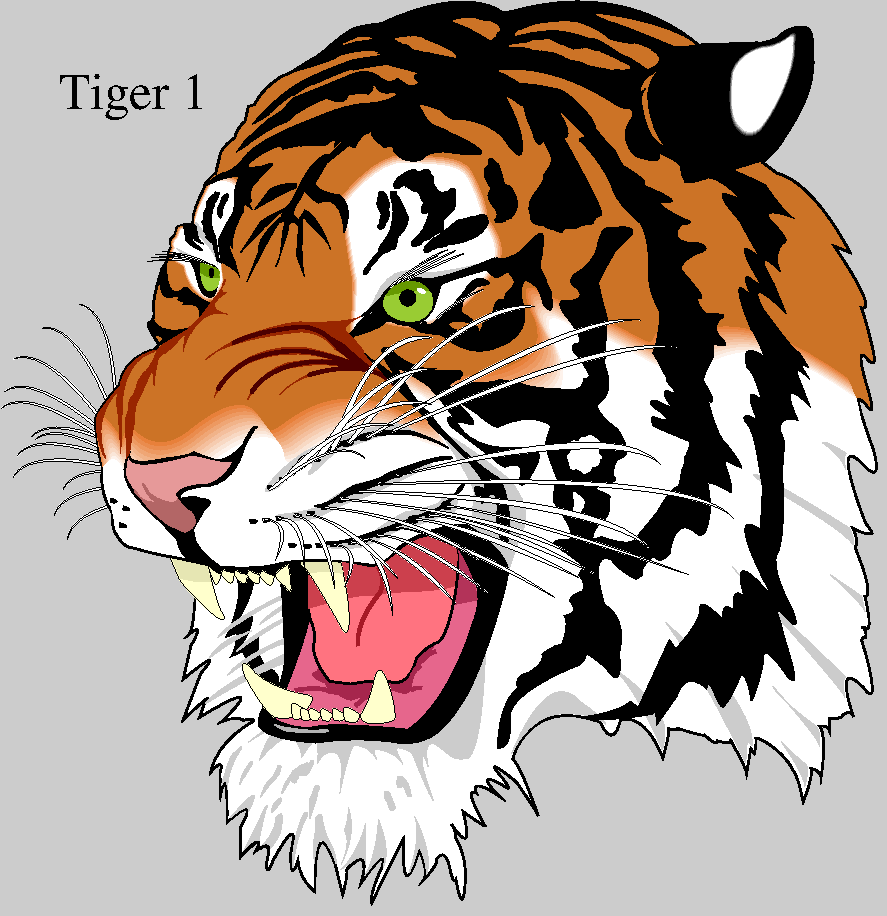
\includegraphics[width=0.5\textwidth]{figure/tiger1.pdf}
    \caption{一枚の図.}
    \label{fig:example}
\end{figure}


\subsection{図を複数枚配置する方法}
\label{ssec:multiple}

\begin{figure}[tp]
    \centering
    \begin{subfigure}{0.45\textwidth}
        \centering
        \includegraphics[width=\textwidth]{example-image-a}
        \caption{左の図.}
        \label{fig:example_a}
    \end{subfigure}
    \hfill % ここで空白を入れると図が適切に配置される
    \begin{subfigure}{0.45\textwidth}
        \centering
        \includegraphics[width=\textwidth]{example-image-b}
        \caption{右の図.}
        \label{fig:example_b}
    \end{subfigure}
    \caption{左右の図.}
    \label{fig:example2}
\end{figure}

\begin{figure}[tp]
    \centering
    % 上の行
    \begin{subfigure}{0.45\textwidth}
        \centering
        \includegraphics[width=\textwidth]{example-image-a}
        \caption{左上の図}
        \label{fig:sub1}
    \end{subfigure}
    \hfill % 水平方向のスペース
    \begin{subfigure}{0.45\textwidth}
        \centering
        \includegraphics[width=\textwidth]{example-image-b}
        \caption{右上の図}
        \label{fig:sub2}
    \end{subfigure}
    
    \vspace{5mm} % 縦方向のスペース
    
    % 下の行
    \begin{subfigure}[b]{0.45\textwidth}
        \centering
        \includegraphics[width=\textwidth]{example-image-c}
        \caption{左下の図}
        \label{fig:sub3}
    \end{subfigure}
    \hfill % 水平方向のスペース
    \begin{subfigure}[b]{0.45\textwidth}
        \centering
        \includegraphics[width=\textwidth]{example-image-c}
        \caption{右下の図}
        \label{fig:sub4}
    \end{subfigure}
    \caption{上下左右に4つ配置された図}
    \label{fig:four_subfigures}
\end{figure}


\ref{fig:four_subfigures}

\ref{fig:sub1}

図~\ref{fig:four_subfigures}(\subref{fig:sub1}--\subref{fig:sub4})
% \subpref{fig:sub1}

\subref{fig:sub1}



\subsection{画像のファイル形式}
\label{ssec:figure_format}



\section{表の配置}
\label{sec:table}






